\documentclass[pdf]{beamer}
%\usepackage{lmodern}
\usepackage[utf8]{inputenc}
\usepackage[english]{babel}
\usepackage{array}

\usepackage{amsmath}
\usepackage{amsthm}
\usepackage{amsfonts}

\usepackage{todonotes}
\usepackage{tikz}
\usetikzlibrary{backgrounds}

\usepackage[backend=bibtex]{biblatex}
\bibliography{masters}

\newcommand{\TODO}{\todo[inline]}
\newcommand{\nstat}{\mathrm{nstat}}
\newcommand{\occu}{\mathrm{occu}}
\newcommand{\go}{\mathrm{go}}
\newcommand{\cont}{\mathrm{cont}}
\newcommand{\stp}{\mathrm{stop}}
\newcommand{\lift}{\mathrm{lift}}
\newcommand{\drop}{\mathrm{drop}}
\newcommand{\edg}{\mathrm{edg}}
\newcommand{\W}{\mathcal{W}}
\newcommand{\Wm}{\mathcal{W}_\mathrm{move}}
\newcommand{\Wmc}{\mathcal{W}_\mathrm{mc}}
\newcommand{\Wl}{\mathcal{W}_\mathrm{lift}}
\newcommand{\Wd}{\mathcal{W}_\mathrm{drop}}
\newcommand{\D}{\mathcal{D}}
\newcommand{\T}{\mathcal{T}}
\newcommand{\td}{\delta}
\newcommand{\tm}{t_{\max}}
\newcommand{\Tn}{\overline{\T}}
\newcommand{\V}{\mathcal{V}}
\newcommand{\E}{\mathcal{E}}
\newcommand{\N}{\mathcal{N}}
\newcommand{\A}{\mathcal{A}}
\newcommand{\B}{\mathcal{B}}

\newcommand{\uw}{\mathrm{uWhat}}
\newcommand{\um}{\mathrm{uMore}}
\newcommand{\ul}{\mathrm{uLess}}
\newcommand{\vl}{\mathrm{vLess}}
\newcommand{\getMC}{\mathrm{getMC}}
\newcommand{\getMT}{\mathrm{getMT}}
\newcommand{\remMC}{\mathrm{remMC}}
\newcommand{\addMC}{\mathrm{addMC}}
\newcommand{\dir}{\mathrm{dir}}
\newcommand{\goOrCont}{\mathrm{goOrCont}}
\newcommand{\contOrStop}{\mathrm{cos}}
\newcommand{\IF}[1]{\text{if}\ #1 \colon}
\newcommand{\IFc}{&\text{if}\ }
\newcommand{\IFco}{&\text{otherwise}}
\newcommand{\away}{\mathrm{away}}
\newcommand{\more}{\mathrm{more}}

\newcommand{\Dn}{North}
\newcommand{\De}{East}
\newcommand{\Ds}{South}
\newcommand{\Dw}{West}

\newcommand{\stat}[1]{\text{\bf #1}}

\newcommand{\testImage}[2]{
    \begin{figure}[h]
        \begin{center}
            \includegraphics[scale=0.7]{fig/#1.png}
            \caption{#2}
        \end{center}
    \end{figure}
}
\newcommand{\ife}{\overset{?}{=}}

\def \myTitle {Integer programming model for automated valet parking}
\def \myTitlE {Täisarvulise planeerimise mudel automaatparklale}

\newtheorem{proposition}{Proposition}

\usetheme{Madrid}
\setbeamertemplate{navigation symbols}{}

\title[IP model for parking]{\myTitle}
\author{Karl Tarbe}
\institute[]{Institute of Computer Science}

\begin{document}
\begin{frame}[plain]
    \titlepage
    \centerline{\scriptsize Supervisor: Dr. Dirk Oliver Theis}
    \hfill 
\includegraphics[width=0.2\textwidth]{fig/ITA_small-logo-eng.png}
\end{frame}

\begin{frame}{Introduction of parking system}
\end{frame}

\begin{frame}{Theoretical results}
    Describe the results from paper~\footfullcite{calinescu2008reconfigurations}.
\end{frame}

\begin{frame}
    \begin{columns}
        \begin{column}{0.4\textwidth}
            \begin{block}{Simultanoues movement}
                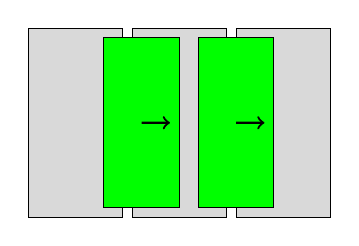
\begin{tikzpicture}[scale=1.2]

\coordinate (A) at (0,2.1);
\coordinate (B) at (1.1,2.1);
\coordinate (C) at (2.2,2.1);


\foreach \v in {A,B,C}
{
    \draw[fill=gray!30] (\v) + (-0.5,-1) rectangle ++(0.5, 1);
}

\coordinate (D) at (0.7, 2.1);
\coordinate (E) at (1.7, 2.1);

\foreach \v in {D,E}
{
    \draw[fill=green] (\v) + (-0.4,-0.9) rectangle ++(0.4, 0.9);
}

\draw[thick,black,->] (D) -- (1,2.1);
\draw[thick,black,->] (E) -- (2,2.1);

\end{tikzpicture}

            \end{block}
        \end{column}
        \begin{column}{0.4\textwidth}
            \begin{block}{Collision from orthogonal direction}
                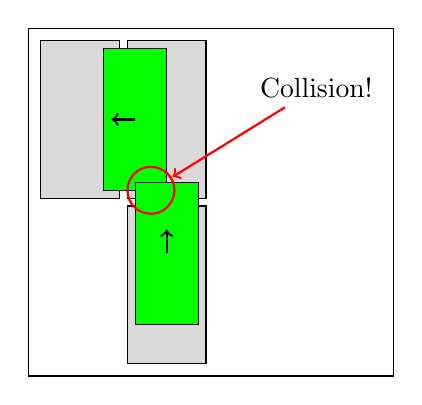
\begin{tikzpicture}[show background rectangle]

\coordinate (A) at (0,2.1);
\coordinate (B) at (1.1,2.1);
\coordinate (C) at (1.1,0);


\foreach \v in {A,B,C}
{
    \draw[fill=gray!30] (\v) + (-0.5,-1) rectangle ++(0.5, 1);
}

\coordinate (D) at (0.7, 2.1);
\coordinate (E) at (1.1, 0.4);

\foreach \v in {D,E}
{
    \draw[fill=green] (\v) + (-0.4,-0.9) rectangle ++(0.4, 0.9);
}

\draw[thick,black,->] (D) -- (0.4,2.1);
\draw[thick,black,->] (E) -- (1.1,0.7);

\node (T) at (3,2.5) {Collision!};
\node[thick, draw, circle, red, scale=1.8] (col) at (0.9,1.2) {};
\draw[thick,red,->] (T) -- (col);

\end{tikzpicture}

            \end{block}
        \end{column}
    \end{columns}
\end{frame}

\begin{frame}{}
\end{frame}

\end{document}
